
\chapter{Calibration of Inertial Measurements} \label{app:A}

The fixed body angular velocities measured by the Inertial Measurement Unit (IMU) are biased due the imperfect orientation of the sensor axis (see \cref{fig:bike_imu}). The goal is  it to allign system xyz with the global coordinate system XYZ. To achieve this the euler angle offesets are calculated by using the measurements from MPU-9050's built in accelerometer. 

\begin{figure}[ht]
    \centering
    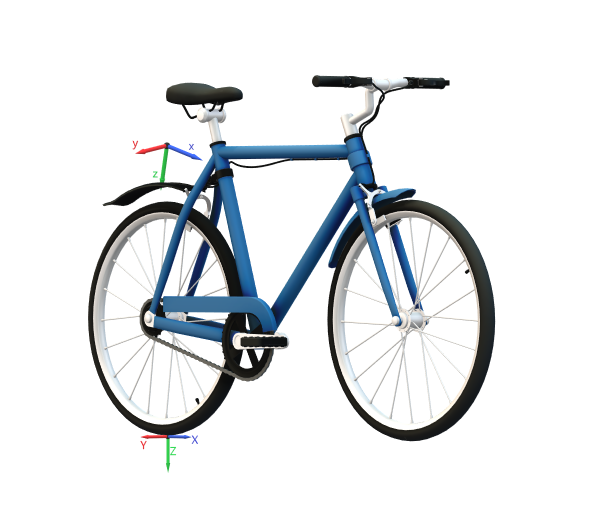
\includegraphics[width=0.7\textwidth]{images/whipple_axis.png}
    \caption{Bicycle with body fixed sensor axis x-y-z (B) and global axis XYZ (G). }
    \label{fig:bike_imu}
\end{figure}

Different orders of rotation affects the end configuration. For this study the intrinsic order Z-Y'-X'' is adopted which is equivalent to the extrinsic X-Y-Z (roll-pitch-yaw). The inverse rotation matrix that described the above rotation sequence is :
\begin{equation}
R_{xyz}=R_x(\phi)R_y(\theta)R_z(\psi)=\left(\begin{array}{ccc}{\cos \theta \cos \psi} & {\cos \theta \sin \psi} & {-\sin \theta} \\ {\cos \psi \sin \theta \sin \phi-\cos \phi \sin \psi} & {\cos \phi \cos \psi+\sin \theta \sin \phi \sin \psi} & {\cos \theta \sin \phi} \\ {\cos \phi \cos \psi \sin \theta+\sin \phi \sin \psi} & {\cos \phi \sin \theta \sin \psi-\cos \psi \sin \phi} & {\cos \theta \cos \phi}\end{array}\right)
    \label{eq:rotmat}
\end{equation}

where \ensuremath{\phi} is the angle of rotation around axis X, \ensuremath{\theta} is the angle of rotation around axis Y and \ensuremath{\psi} is the angle of rotation around axis Z. \Cref{eq:rotmat} maps a vector from the global system G to the body fixed system B. In order to estimate the euler angle offsets the bike was configured in two different ways to aligne the gravity vector with the z and x axis respectively.
The readings from the accelerometer are expressed in the sensor frame (B). \Cref{eq:firstIMU}  is used to solve for the euler angle offsets. Unfortunately the three equations have only two degrees of freedom so two configurations are required so as to solve for all three angles. 

 In the first, \ensuremath{i=1} and \ensuremath{\boldsymbol{g}_1=[ 0 \;\; 0 \;\; 1]^T } (see) with \cref{eq:firstIMU} solving for \ensuremath{\theta} and \ensuremath{\phi}. The lack of any dependence on the yaw  angle is intuitive to understand since a rotation  around the z-axis is aligned with the gravitational field and accelerometers are completely insensitive to rotations about the gravitational field vector. Consequently in the second, \ensuremath{i=2} and \ensuremath{\boldsymbol{g}_2=[ -1 \;\;0\;\; 0 ]^T} which leads to   \cref{eq:firstIMU} solving for \ensuremath{\psi} and \ensuremath{\theta} (see).
 
 \begin{equation}
 \frac{\boldsymbol{G}_{i}^B}{\norm{\boldsymbol{G}_{i}^B}}=\left(\begin{array}{l}{G_{i x}^B} \\ {G_{i y}^B} \\ {G_{i z}^B}\end{array}\right)\frac{1}{\sqrt{{G_{i x}^B}^2+{G_{i y}^B}^2+{G_{i z}^B}^2}}=R_{\mathit{xyz}}\boldsymbol{g}_i
\label{eq:firstIMU}
 \end{equation}
 
Solving \cref{eq:firstIMU} for the angles we get :
\begin{align}
   & \phi=tan^{-1}\left(\frac{G_{1x}^B}{G_{1y}^B}\right)
   \label{eq:offset1}
   \\
   & \theta= tan^{-1}\left(\frac{G_{1 x}^B}{\sqrt{{G_{1 y}^B}^{2}+{G_{1 z}^B}^{2}}}\right) 
   \\
   & \psi = tan^{-1}\left(\frac{-G_{2 y}^B}{\sqrt{{G_{2 x}^B}^{2}+{G_{2 z}^B}^{2}}}\right)
   \label{eq:offset3}
\end{align}

From \crefrange{eq:offset1}{eq:offset3} the euler angle offsets calculated are inserted into rotation matrix \ensuremath{R_{\mathit{xyz}}}. The transpose of the result (\ref{eq:resultIMU}) is then used to transform the IMU measurements from the coordinate frame B to the coordinate frame G which is consistent with the linearized equations of motion defined in \cref{subsec:EOM}.

\begin{equation}
R_{\mathit{xyz}}^T=\left(\begin{array}{ccc} 0.9939 & -0.006106 & -0.1105\\ 0.006069 & 1.0 & -0.000675\\ 0.1105 & 0 & 0.9939 \end{array}\right)
    \label{eq:resultIMU}
\end{equation}